\documentclass[conference]{IEEEtran}

\usepackage{cite}
\usepackage{amsmath,amssymb,amsfonts}
\usepackage{graphicx}
\usepackage{textcomp}
\usepackage{xcolor}
\usepackage{booktabs}
\usepackage{array}
\usepackage{microtype}
\PassOptionsToPackage{hyphens}{url}
\usepackage[hidelinks]{hyperref}
\urlstyle{tt}
\renewcommand{\dbltopfraction}{0.85}
\renewcommand{\topfraction}{0.85}
\renewcommand{\textfraction}{0.10}
\renewcommand{\floatpagefraction}{0.50}
\renewcommand{\dblfloatpagefraction}{0.50}
\setlength{\dbltextfloatsep}{10pt plus 2pt minus 2pt}
\setlength{\dblfloatsep}{8pt plus 2pt minus 2pt}
\setlength{\textfloatsep}{10pt plus 2pt minus 2pt}
\setlength{\abovecaptionskip}{4pt}
\setlength{\belowcaptionskip}{0pt}

% Center second row of 5 authors cleanly in IEEEtran conference mode
\makeatletter
\newcommand{\linebreakand}{%
  \end{@IEEEauthorhalign}
  \hfill\mbox{}\par
  \mbox{}\hfill\begin{@IEEEauthorhalign}
}
\makeatother

\begin{document}

\title{SunSync-AI: Machine Learning-Driven Solar Nowcasting and Computer Vision for Proactive Smart Film Shading Control}

\author{
\IEEEauthorblockN{Jiyeon Kim}
\IEEEauthorblockA{\textit{Dept. of Information Systems}\\
\textit{Hanyang University}\\
Seoul, South Korea\\
kjy8402@hanyang.ac.kr}
\and
\IEEEauthorblockN{Daeun Lee}
\IEEEauthorblockA{\textit{Dept. of Information Systems}\\
\textit{Hanyang University}\\
Seoul, South Korea\\
daeun4862@hanyang.ac.kr}
\and
\IEEEauthorblockN{Dain Lee}
\IEEEauthorblockA{\textit{Dept. of Information Systems}\\
\textit{Hanyang University}\\
Seoul, South Korea\\
ldi0308@hanyang.ac.kr}
\linebreakand
\IEEEauthorblockN{Heegyeong Chung}
\IEEEauthorblockA{\textit{Dept. of Information Systems}\\
\textit{Hanyang University}\\
Seoul, South Korea\\
hgchung04@gmail.com}
\and
\IEEEauthorblockN{Misong Ha}
\IEEEauthorblockA{\textit{Dept. of Information Systems}\\
\textit{Hanyang University}\\
Seoul, South Korea\\
msha9865@hanyang.ac.kr}
}

\maketitle

\begin{abstract}
Libraries, archives, museums, and sunlit workspaces face a recurring conflict between preserving light-sensitive materials from photodegradation and maintaining natural daylight. Conventional motorized blinds and uniform dynamic glazing react only after exposure begins and darken entire windows regardless of interior furniture layout. This work presents SunSync-AI, an integrated prototype service that combines deterministic three-dimensional ray tracing with three applied machine learning and computer vision pipelines for cell-level smart window film control. First, a physically bounded linear quantile regression nowcaster trained on 28 days of Korea Meteorological Administration GK2A satellite observations and archived Open-Meteo forecasts reduces 10-minute and 30-minute direct normal irradiance mean absolute error by 56.2 percent and 26.8 percent on a strict four-day holdout test, achieving 81.1 percent empirical coverage at the 10-minute horizon. Second, a coarse-to-fine vision sensing pipeline fuses pretrained YOLOv8 object detection, Depth Anything V2 Metric Indoor monocular depth estimation, EXIF and 1D-search ArUco camera pose recovery, proportional inner-60\% single-marker calibration, and 3D ENU point-cloud cuboid fitting; evaluated across 11 depth model variants and four capture conditions in a tape-measured $3.30 \times 4.10 \times 2.50\text{ m}$ room, our production fixes cut live end-to-end wall-normal depth MAE by 65.3 percent (0.557 m to 0.193 m), raise desk 2D footprint IoU by 69.0 percent (0.289 to 0.489), and remove 90.9 percent of confirmed false positives at zero additional model weight. Third, an uncertainty-aware adaptive film controller suppresses up to 65.9 percent of switching events on measured one-minute intermittent irradiance streams while admitting over 31 percent more daylight than coarse 30-minute rule schedules, supported by a 10-minute rolling scenario precomputation architecture.
\end{abstract}

\begin{IEEEkeywords}
Solar irradiance nowcasting, quantile regression, monocular 3D estimation, ArUco pose calibration, adaptive smart glazing control, switchable glazing film.
\end{IEEEkeywords}

\section{Introduction}

\subsection{Motivation}
Sunlit reading rooms, archives, and museum galleries must balance two competing objectives: preventing ultraviolet and high-intensity direct sunlight from damaging sensitive books or exhibits, and preserving natural daylight for human occupants. Conventional motorized blinds and full-pane electrochromic windows operate reactively after glare occurs and darken the entire glazed area even when a solar beam intersects only a single bookshelf or desk.

Inspired by LG Chem Switchable Glazing Film (SGF) and the LG ThinQ ON smart-home ecosystem, we developed \textbf{SunSync-AI} (\url{https://github.com/hing9-9-9/SunSync}). SunSync partitions each window into a discrete grid of individually addressable cells (up to $10 \times 10$ per film module) and traces three-dimensional solar rays from the window plane to protected interior surfaces. Only the cells whose ray paths intersect a protected region above its irradiance threshold are darkened, as shown in Fig.~\ref{fig:3dview}.

\begin{figure}[t]
\centering
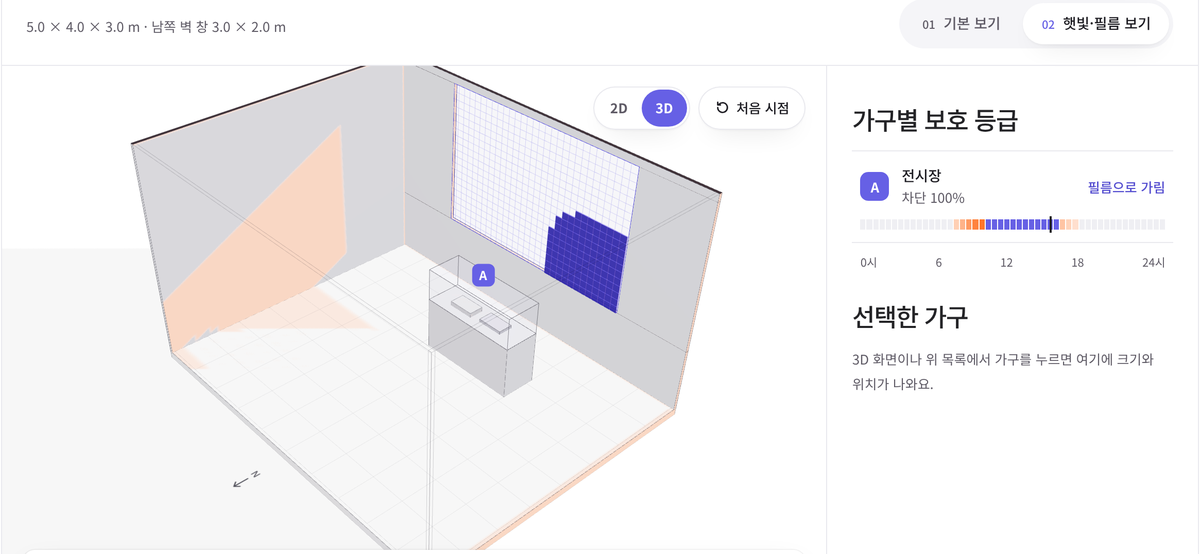
\includegraphics[width=\columnwidth]{../images/readme-3d-view.png}
\caption{Live SunSync 3D prototype view ($5.0 \times 4.0 \times 3.0\text{ m}$ room, south window). Only the specific blue film cells blocking direct solar rays onto the Grade A display case are darkened while surrounding cells remain transparent.}
\label{fig:3dview}
\end{figure}

\begin{table*}[t]
\caption{SunSync-AI Implemented Capabilities and Verification Artifacts (\texttt{main@882521e})}
\label{tab:scope}
\centering
\footnotesize
\setlength{\tabcolsep}{5pt}
\renewcommand{\arraystretch}{1.15}
\begin{tabular}{@{} >{\raggedright\arraybackslash}p{0.19\textwidth} >{\raggedright\arraybackslash}p{0.43\textwidth} >{\raggedright\arraybackslash}p{0.33\textwidth} @{}}
\toprule
\textbf{AIML Track} & \textbf{Implemented Capabilities on \texttt{main}} & \textbf{Primary Code Artifacts} \\
\midrule
Track 1: Solar Nowcasting (\texttt{FR-01.4}) &
Frozen \texttt{fr01\_kma\_quantile\_v1} trained on 28 days of KMA GK2A and Open-Meteo data; one-time 4-day holdout evaluated; operational shadow worker and UI daylight provenance bar. &
\path{server/backend/app/nowcast/}, \path{model_artifacts/fr01_kma_quantile_v1/}, \path{frontend/src/weatherProvenance.ts} \\
Track 2: Vision AI 3D Sensing (\texttt{FR-03}/\texttt{FR-06}) &
In-app single-photo scan, EXIF \& 1D-search ArUco pose, YOLOv8m (deterministic FP gates) + Depth Anything V2 Metric Small ($\le 1024\text{ px}$, proportional calibration, 3D ENU point-cloud cuboids, non-destructive clamping), 2D \texttt{VisionPreview}, Guided ArUco \texttt{P1}--\texttt{P4}, and \texttt{mode=experiment} diagnostics. &
\path{server/engine/vision_ai/}, \path{server/backend/app/api/vision_ai.py}, \path{server/backend/app/services/film.py}, \path{frontend/src/VisionPreview.tsx}, \path{visualize_fr03_pipeline.py} \\
Track 3: Adaptive Control (\texttt{FR-04}) and Precomputation &
Default \texttt{smooth\_fr02} API stabilization, Viterbi DP \texttt{replace} mode (binary PDLC and 5-level LG SGF), ThinQ ON bridge contract, real KMA and 1-min NOAA SURFRAD replays, and 10-min rolling scenario precomputation. &
\path{server/engine/fr04/}, \path{docs/experiments/fr04_*}, \path{scenario_store.py}, \path{GET /api/scenes/{id}/scenario} \\
\bottomrule
\end{tabular}
\end{table*}

Deterministic geometric ray tracing alone leaves three operational problems unresolved:
\begin{enumerate}
\item \textit{Sub-hourly cloud transients:} Hourly Numerical Weather Prediction (NWP) feeds lag fast cumulus passages, causing either unshaded irradiance spikes or prolonged unnecessary darkening.
\item \textit{Indoor 3D setup friction:} Manually measuring East-North-Up (ENU) furniture coordinates slows deployment, whereas single-photo monocular depth models suffer from scale ambiguity and 20 to 40~cm 3D localization error.
\item \textit{Cloud-induced film flicker:} Toggling binary cells whenever forecasted Direct Normal Irradiance (DNI) crosses a fixed threshold causes visual flicker and accelerates switching wear.
\end{enumerate}

\subsection{Implemented System Scope}
SunSync-AI addresses all three gaps inside one FastAPI, SQLite, and React/Three.js application (codebase reference \texttt{main@882521e}). Table~\ref{tab:scope} summarizes the implemented AIML tracks and verification artifacts.

\section{Datasets}

We assembled and audited three dataset suites with explicit SHA-256 checksums, UTC timestamps, and temporal leakage controls.

\subsection{Solar Irradiance Nowcasting Dataset (FR-01.4)}
For Seoul ($37.5714^\circ\text{ N}, 126.9658^\circ\text{ E}$), we paired 10-minute geostationary satellite point observations from the Korea Meteorological Administration (KMA) GK2A API Hub \cite{b8} with archived historical NWP runs from Open-Meteo (\texttt{ecmwf\_ifs025}) \cite{b9}. Table~\ref{tab:fr01_data} details the development and frozen final-test inputs.

\begin{table*}[t]
\caption{FR-01.4 KMA GK2A and Open-Meteo Archived Forecast Dataset Specification}
\label{tab:fr01_data}
\centering
\footnotesize
\setlength{\tabcolsep}{4.5pt}
\renewcommand{\arraystretch}{1.12}
\begin{tabular}{@{}llllll@{}}
\toprule
\textbf{Dataset Component} & \textbf{Source and Resolution} & \textbf{UTC Period} & \textbf{Rows / Runs} & \textbf{SHA-256} & \textbf{Role} \\
\midrule
Development KMA & GK2A \texttt{DSR}, \texttt{CA} (10-min) & 2026-10-05--11-01 (28~d) & 4,032 rows & \texttt{00e8259d5dbb} & Train / Val / Diag \\
Development Open-Meteo & \texttt{ecmwf\_ifs025} (6-h, hourly) & 2026-10-05--11-01 & 3,192 (114 runs) & \texttt{484e7b97d0ba} & Prior \& baseline \\
Final Test KMA & GK2A \texttt{DSR}, \texttt{CA} (10-min) & 2026-11-02--11-05 (4~d) & 576 rows & \texttt{838bf1c4e0c2} & Frozen final test \\
Final Test Open-Meteo & \texttt{ecmwf\_ifs025} (6-h runs) & 2026-11-01 12Z--11-05 18Z & 504 (18 runs) & \texttt{1f2a3f841237} & Holdout (+7~h) \\
\bottomrule
\end{tabular}
\end{table*}

\textbf{Anti-Leakage Split Contract.} Open-Meteo forecasts represent \texttt{preceding\_hour\_mean} values anchored to each issuance run (\texttt{issued\_at\_utc}). Our dataset builder enforces an availability delay of \texttt{issued\_at\_utc + 7 hours} and a chronological embargo (\texttt{valid\_time < next\_split\_start}) across four partitions:
\begin{itemize}
\item \textit{Train (Oct.~5--28 UTC):} 1,266 / 1,216 / 1,141 valid daylight rows for 10 / 30 / 60-minute horizons.
\item \textit{Validation (Oct.~29--30 UTC):} 97 / 91 / 82 rows, used exclusively for specification and bound selection.
\item \textit{Diagnostic (Oct.~31--Nov.~1 UTC):} 97 / 91 / 82 rows, report-only and excluded from model selection.
\item \textit{Frozen Final Test (Nov.~2--5 UTC):} 180 / 168 / 151 valid daylight rows evaluated once after freezing V1.
\end{itemize}

\textbf{Data Quality Audit.} Verification confirmed zero duplicate timestamps and zero 10-minute cadence breaks. Provider missing sentinels (\texttt{nan}, \texttt{6553.5}, negative flags) and four out-of-range cloud-amount records (\texttt{1.1}) were normalized to null rather than zero-imputed. Nighttime rows (solar elevation below $5^\circ$) accounted for most DSR nulls (2,512 excluded input rows across 28 days), alongside occasional daytime satellite outages (173 daytime nulls in the initial 14-day audit). Valid daytime DSR and cloud amount correlated at Pearson $r = -0.657$. Because KMA supplies downward shortwave radiation (\texttt{DSR}) rather than DNI, we convert \texttt{DSR} to a solar-geometry-corrected DNI reference (\texttt{dsr\_proxy}) using the Erbs decomposition \cite{b1} in \texttt{pvlib} \cite{b4}.

\subsection{Real-Weather and 1-Minute Replay Datasets (FR-04)}
To test adaptive control under realistic cloud intermittency, we assembled three complementary FR-04 testbeds:
\begin{enumerate}
\item \textit{Synthetic 4-Scenario Stress Suite:} 5-minute steps (08:00--18:00) over a $4 \times 4$ south window (1 Grade A cell, 3 Grade B cells capped at $30\text{ W/m}^2$, 12 Grade D cells) across \texttt{Sunny}, \texttt{Partly Cloudy Rapid-Flicker}, \texttt{High Uncertainty Squall}, and \texttt{Overcast} skies.
\item \textit{Real KMA GK2A 10-Minute Replay:} Four Seoul days from the development set (\texttt{2026-10-10} clear, mean DSR $529.2\text{ W/m}^2$; \texttt{2026-10-16} intermittent, 15 cloud flips; \texttt{2026-10-05} restless intermittent, 13 DSR jumps $\ge 150\text{ W/m}^2$; \texttt{2026-10-18} overcast, $112.7\text{ W/m}^2$; 206 records replayed at 5, 10, and 30-min steps).
\item \textit{Real 1-Minute Measured DNI Replay:} Four quality-flag-0 one-minute DNI days from NOAA SURFRAD (\texttt{Penn\_State\_PA}) \cite{b10} mapped by solar time onto our Seoul scene (\texttt{2023-10-11} clear, $829\text{ W/m}^2$; \texttt{2023-10-02} intermittent sunny, 32 crossings of $100\text{ W/m}^2$; \texttt{2023-10-22} restless intermittent, 83 crossings of $100\text{ W/m}^2$, 90 jumps $\ge 300\text{ W/m}^2$, and 39 dips under 10~min; \texttt{2023-10-06} overcast).
\end{enumerate}

\subsection{Vision AI 3D Benchmark and Field Inputs (FR-03 and FR-06)}
Object detection uses pretrained COCO-80 \texttt{yolov8m.pt} \cite{b7} mapped to SunSync classes (\texttt{bookshelf}, \texttt{desk}, \texttt{chair}, \texttt{other}) paired with \path{Depth-Anything-V2-Metric-Indoor-Small-hf} \cite{b6} and a window-mounted $6 \times 6$ ArUco \texttt{DICT\_4X4\_50} marker ($s = 0.6\text{ m}$). For synthetic noise sweeps, \texttt{run\_fr03\_vision\_3d\_experiment.py} models a $6.0 \times 5.0 \times 2.8\text{ m}$ reading room with a north window marker at $(3.0, 5.0, 1.6)\text{ m}$ and three floor-standing objects: Library Bookshelf ($1.20 \times 0.40 \times 1.80\text{ m}$), Oak Study Desk ($1.40 \times 0.70 \times 0.75\text{ m}$), and Ergonomic Chair ($0.60 \times 0.60 \times 0.85\text{ m}$). For physical field validation, we collected the \texttt{depthtest} benchmark in a tape-measured $3.30 \times 4.10 \times 2.50\text{ m}$ room with a glass corridor wall at $x = 3.30\text{ m}$ and a north marker wall at $y = 4.10\text{ m}$ ($d_{\mathrm{wall}} = 4.10 - y_{\mathrm{ENU}}$). Five smartphone images span four conditions (\texttt{original} 1$\times$, \texttt{distortion} 0.5$\times$ ultrawide, \texttt{otherside} opposite view facing the glass wall, and portrait \texttt{twochair} on Galaxy S23+ with \texttt{Orientation=6}; three images have EXIF stripped). A $0.60\text{ m}$ ArUco marker (\texttt{code\_id=31}, center $(1.50, 4.10, 1.50)\text{ m}$, verified by $z = 0.76\text{ m}$ ray-plane intersection) anchors $N=6$ primary targets: a desk ($1.20\text{ m}$ parallel $\times 1.78\text{ m}$ perpendicular $\times 0.76\text{ m}$ height, front $1.17\text{ m}$, center $2.06\text{ m}$) across four desk photos plus a blue chair ($1.17\text{ m}$) and white chair ($1.80\text{ m}$, both $0.47 \times 0.46 \times 0.80\text{ m}$) in \texttt{twochair}.

\section{Methodology}

\subsection{End-to-End Architecture}
Fig.~\ref{fig:arch} illustrates how the three AIML pipelines connect inside the live service. Track 2 registers 3D ENU occluders and protected regions into the Scene store, Track 1 forecasts sub-hourly probabilistic DNI, and Track 3 combines cached 3D ray intersections with weather fingerprints to maintain precomputed shading plans.

\begin{figure*}[t]
\centering
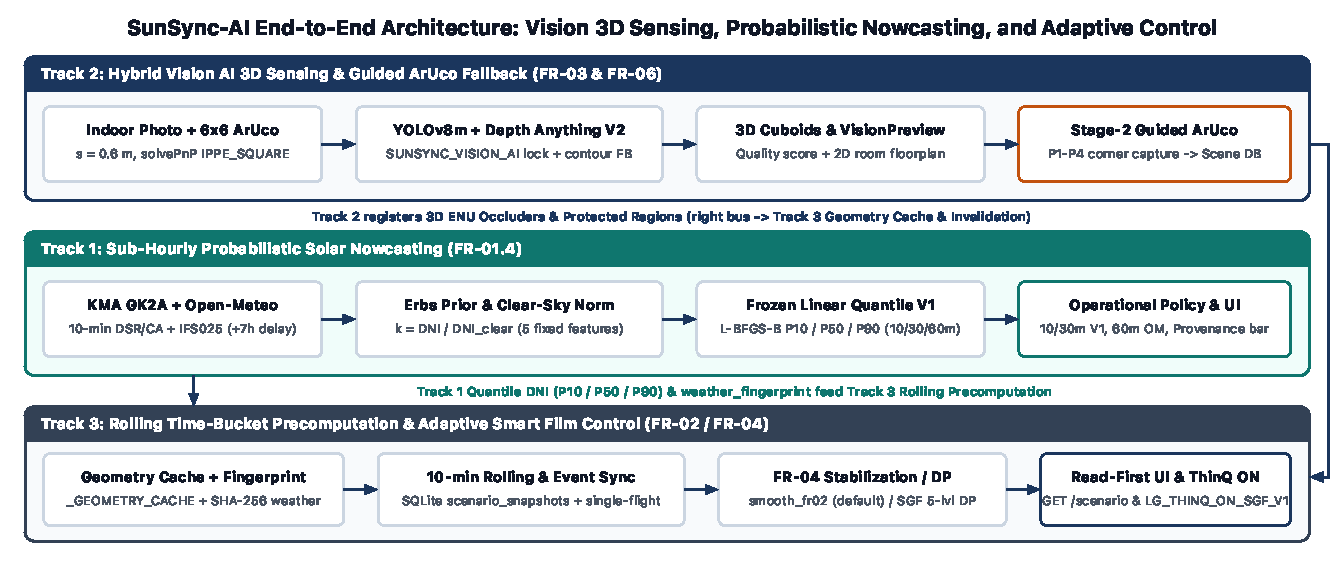
\includegraphics[width=0.84\textwidth]{figures/fig0_system_architecture.pdf}
\caption{End-to-end SunSync-AI architecture connecting Track 2 (Hybrid Vision AI 3D sensing and Guided ArUco fallback), Track 1 (FR-01.4 sub-hourly quantile solar nowcasting), and Track 3 (10-minute rolling precomputation and FR-04 adaptive smart-film control).}
\label{fig:arch}
\end{figure*}

\subsection{Track 1: Sub-Hourly Probabilistic Solar Nowcasting}
\textbf{Algorithm Choice.} Auditing our 28-day development set ($\approx 1{,}200$ valid daylight rows per horizon) showed that high-capacity nonlinear models risk overfitting one autumn season. We therefore selected \textbf{physically bounded Linear Quantile Regression} ($P_{10}, P_{50}, P_{90}$) trained in clear-sky-normalized space with \texttt{scipy.optimize} (L-BFGS-B) for frozen model \texttt{fr01\_kma\_quantile\_v1}. Each horizon serializes into a 5~KB JSON artifact with sub-millisecond CPU inference and $0.0\text{ W/m}^2$ round-trip serialization error.

\textbf{Feature Formulation.} Instead of regressing raw irradiance, each model predicts the dimensionless clear-sky ratio $k_q = \mathrm{DNI}_q / \mathrm{DNI}_{\mathrm{clear}}$ from five fixed features: \texttt{intercept} ($1.0$), lead-time blended \texttt{direct\_prior\_factor} $x_{\mathrm{prior}}$, \texttt{open\_meteo\_factor} ($\mathrm{OM\_DNI}/\mathrm{DNI}_{\mathrm{clear}}$), \texttt{cloud\_transmittance} ($1 - \mathrm{CA}/100$), and \texttt{advection\_impact} (fixed at $0.0$ in V1 for future cloud-motion patches):
\begin{align}
w_{\mathrm{obs}}(h) &= \exp\!\left(-\frac{h/60}{1.5}\right), \nonumber\\
x_{\mathrm{prior}} &= w_{\mathrm{obs}} k_{\mathrm{erbs}} + (1 - w_{\mathrm{obs}}) k_{\mathrm{om}},
\label{eq:prior}
\end{align}
where $h \in \{10, 30, 60\}$ minutes, $k_{\mathrm{erbs}} = \mathrm{KMA\_DNI}_{\mathrm{prior}} / \mathrm{DNI}_{\mathrm{clear}}$, and $k_{\mathrm{om}} = \mathrm{OM\_DNI} / \mathrm{DNI}_{\mathrm{clear}}$. Postprocessing guarantees physical bounds and monotonicity:
\begin{align}
\hat{k}_{10} &= \mathrm{clip}\big(f_{10}(\mathbf{x}), 0, 1.05\big), \nonumber\\
\hat{k}_{50} &= \max\!\big(\hat{k}_{10}, \mathrm{clip}(f_{50}(\mathbf{x}), 0, 1.05)\big), \nonumber\\
\hat{k}_{90} &= \max\!\big(\hat{k}_{50}, \mathrm{clip}(f_{90}(\mathbf{x}), 0, 1.05)\big).
\label{eq:mono}
\end{align}

Table~\ref{tab:weights} reports the exact frozen weights. At 10~minutes, $P_{50}$ places nearly unit weight ($1.008$) on $x_{\mathrm{prior}}$ (recent satellite persistence), whereas at 60~minutes $P_{10}$ shifts away from persistence ($0.000$) onto \texttt{open\_meteo\_factor} ($0.508$) and \texttt{cloud\_transmittance} ($0.347$). For 60-minute $P_{90}$, we kept the $[-0.5, 0.5]$ intercept bound because it outperformed $[-0.75, 0.75]$ on validation $P_{90}$ pinball loss ($42.14$ vs.\ $42.51\text{ W/m}^2$) and interval width ($452.96$ vs.\ $493.81\text{ W/m}^2$). In operations (\texttt{kma\_operational.py}), 10 and 30-minute horizons serve frozen V1, 60~minutes serves Open-Meteo (logging V1 in shadow), stale ($>20\text{ min}$) or missing KMA triggers Open-Meteo fallback, and \texttt{weatherProvenance.ts} displays daylight forecast coverage in the UI.

\begin{figure*}[t]
\centering
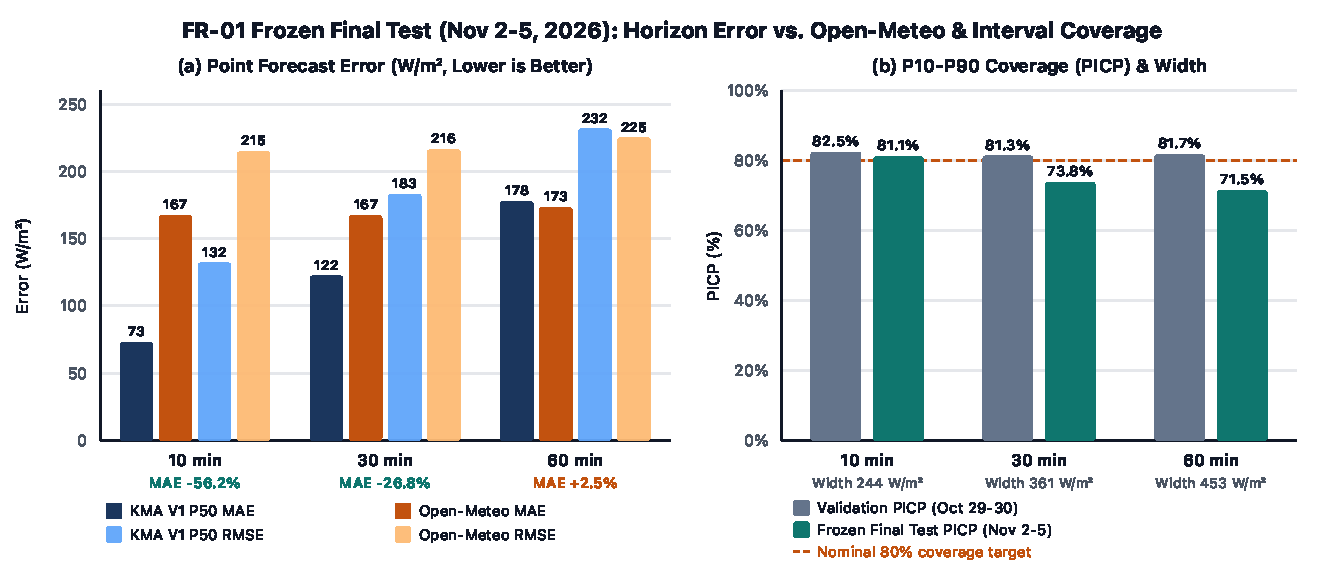
\includegraphics[width=0.82\textwidth]{figures/fig1_fr01_horizon_error.pdf}
\caption{FR-01 frozen V1 (\texttt{fr01\_kma\_quantile\_v1}) one-time Final Test (Nov.~2--5, 2026) point forecast MAE and RMSE versus Open-Meteo ECMWF IFS025 (a), and $P_{10}$--$P_{90}$ Prediction Interval Coverage Probability (PICP) with mean interval width across Validation and Final Test (b).}
\label{fig:fr01_err}
\end{figure*}

\begin{table}[t]
\caption{Frozen V1 Linear Quantile Regression Weights (\texttt{advection\_impact} $= 0$)}
\label{tab:weights}
\centering
\renewcommand{\arraystretch}{1.08}
\begin{tabular}{@{}ccrrrr@{}}
\toprule
\textbf{Horizon} & \textbf{Quantile} & \textbf{Bias} & \textbf{Prior} & \textbf{OM} & \textbf{Cloud} \\
\midrule
10~min & $P_{10}$ & $-0.132$ & $0.583$ & $0.000$ & $0.384$ \\
10~min & $P_{50}$ & $-0.005$ & $1.008$ & $0.000$ & $0.016$ \\
10~min & $P_{90}$ & $0.364$  & $0.757$ & $0.000$ & $-0.079$ \\
\midrule
30~min & $P_{10}$ & $-0.130$ & $0.277$ & $0.122$ & $0.463$ \\
30~min & $P_{50}$ & $-0.002$ & $0.897$ & $0.017$ & $0.120$ \\
30~min & $P_{90}$ & $0.469$  & $0.710$ & $0.000$ & $-0.090$ \\
\midrule
60~min & $P_{10}$ & $-0.177$ & $0.000$ & $0.508$ & $0.347$ \\
60~min & $P_{50}$ & $-0.016$ & $0.824$ & $0.000$ & $0.214$ \\
60~min & $P_{90}$ & $0.500$  & $0.698$ & $0.000$ & $-0.051$ \\
\bottomrule
\end{tabular}
\end{table}

\subsection{Track 2: Hybrid Vision AI 3D Sensing and Guided ArUco Fallback}
Single-photo monocular depth networks lack stable absolute scale across smartphone focal lengths (0.5$\times$ ultrawide vs.\ 1$\times$ wide). Informed by our real-room ablation study (Section~\ref{sec:fr03_eval}), SunSync anchors every photograph to the paired $6 \times 6$ window ArUco marker ($s = 0.6\text{ m}$):
\begin{enumerate}
\item \textit{EXIF Intrinsics, 1D Focal Search, and Metric Pose:} Image decoding applies EXIF orientation transpose and extracts \texttt{FocalLengthIn35mmFilm} (with optional \texttt{fov\_deg}/\texttt{focal\_length\_35mm} overrides) rather than hardcoding $f_x = 0.9\max(w, h)$. When EXIF is stripped, initialization starts at $0.68\max(w, h)$ and, if \texttt{SOLVEPNP\_IPPE\_SQUARE} \cite{b5} reprojection error exceeds $2.5\text{ px}$ or the camera falls outside \texttt{room\_floor\_poly.buffer(0.25)}, runs a 1D search over $f_x / \max(w, h) \in [0.35, 0.90]$ minimizing reprojection error while keeping the camera inside the room:
\begin{align}
R_{\mathrm{ENU},c} &= R_{\mathrm{ENU},m} R_{c,m}^{\mathsf{T}}, \nonumber\\
t_{\mathrm{ENU},c} &= t_{\mathrm{ENU},m} - R_{\mathrm{ENU},c} t_{c,m}.
\label{eq:pose}
\end{align}
\begin{table*}[t]
\caption{FR-01 Validation (Oct.~29--30) and One-Time Frozen Final Test (Nov.~2--5, 2026) Metrics vs.\ Open-Meteo (W/m\textsuperscript{2})}
\label{tab:fr01_eval}
\centering
\footnotesize
\setlength{\tabcolsep}{4.5pt}
\renewcommand{\arraystretch}{1.10}
\begin{tabular}{@{}lcrrrrrrrrr@{}}
\toprule
\textbf{Split} & \textbf{Horizon} & \textbf{Rows} & \textbf{V1 $P_{50}$ MAE} & \textbf{OM MAE} & \textbf{MAE $\Delta$} & \textbf{V1 RMSE} & \textbf{OM RMSE} & \textbf{$P_{50}$ Pinball} & \textbf{PICP (80\%)} & \textbf{Width} \\
\midrule
Validation & 10~min & 97  & \textbf{62.29}  & 163.94 & $-62.0\%$ & \textbf{122.23} & 208.71 & 31.14 & 82.5\% & 272.72 \\
Validation & 30~min & 91  & \textbf{83.62}  & 159.20 & $-47.5\%$ & \textbf{133.15} & 205.58 & 41.81 & 81.3\% & 381.67 \\
Validation & 60~min & 82  & \textbf{117.43} & 157.34 & $-25.4\%$ & \textbf{181.84} & 205.94 & 58.71 & 81.7\% & 452.96 \\
\midrule
\textbf{Final Test} & \textbf{10~min} & 180 & \textbf{73.16}  & 167.19 & $\mathbf{-56.2\%}$ & \textbf{131.98} & 214.63 & 36.58 & \textbf{81.1\%} & 244.41 \\
\textbf{Final Test} & \textbf{30~min} & 168 & \textbf{122.30} & 167.16 & $\mathbf{-26.8\%}$ & \textbf{183.05} & 216.10 & 61.15 & 73.8\% & 361.07 \\
\textbf{Final Test} & \textbf{60~min} & 151 & 177.54 & \textbf{173.25} & $+2.5\%$ & 231.59 & \textbf{224.98} & 88.77 & 71.5\% & 453.31 \\
\bottomrule
\end{tabular}
\end{table*}
\begin{figure*}[t]
\centering
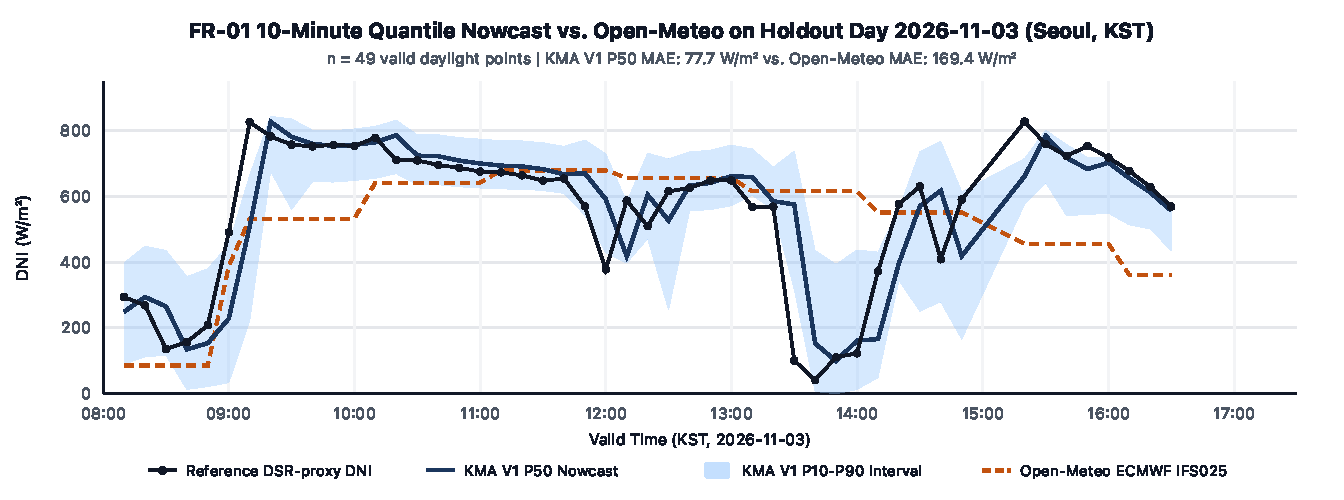
\includegraphics[width=0.80\textwidth]{figures/fig2_fr01_timeseries_10min.pdf}
\caption{10-minute probabilistic nowcast versus Open-Meteo ECMWF IFS025 on holdout Final Test day \texttt{2026-11-03} (Seoul, KST, $n=49$ valid daylight points). KMA V1 tracks the 13:20--14:10 KST cloud drop missed by hourly NWP (daily MAE $77.7$ vs.\ $169.4\text{ W/m}^2$).}
\label{fig:fr01_ts}
\end{figure*}
\item \textit{Proportional Single-Marker Calibration:} Fitting a two-parameter affine line ($\alpha d + \beta$) to four coplanar marker corners overfits marker noise and extrapolates wild intercepts ($\beta \in [-2.12, +0.92]\text{ m}$). \texttt{calibrate\_monocular\_depth} therefore defaults to proportional scaling ($\beta = 0$) from the inner-60\% marker quad median, enabling affine fitting only when multi-depth anchors span $\mathrm{ptp}(Z_{\mathrm{true}}) \ge 1.5\text{ m}$.
\item \textit{Deterministic FP Gates and 3D ENU Point-Cloud Cuboids:} \texttt{YoloV8DetectorAdapter} (\texttt{conf\_thresh} $= 0.25$) applies class-agnostic NMS ($\mathrm{IoU} \ge 0.65$), requires $\ge 3$ clustered \texttt{book} detections to emit \texttt{bookshelf}, excludes \texttt{tv}/\texttt{other} boxes containing $\ge 80\%$ of the marker box, and drops detections whose unclamped ENU center lies outside \texttt{room\_floor\_poly.buffer(0.25)}. \texttt{MonocularDepthAdapter} resizes inputs to $\le 1024\text{ px}$ under \texttt{torch.inference\_mode()} and runs even when clients supply \texttt{request.detections}. \texttt{backproject\_box\_to\_3d\_cuboid} unprojects a strided 3D ENU point cloud (\texttt{enu\_pointcloud\_bbox}, inner 80\% box), applies foreground filtering ($z \ge 0.10\text{ m}$, nearest 65\% for chairs, $z \in [0.20, 1.30]\text{ m}$ for desks), aligns yaw to room walls, fits robust $p_5$--$p_{95}$ extents with floor-referenced top height ($p_{\mathrm{top,ENU},z}$), and applies non-destructive \texttt{clamp\_cuboid\_to\_room} (minimal inward translation first).
\item \textit{Coarse-to-Fine Hybrid Capture UX:} \texttt{\_assess\_estimation\_quality} grades each item (\texttt{high}, \texttt{medium}, or \texttt{low\_needs\_aruco}), reports perpendicular window-wall distance ($d_{\mathrm{window}}$) in capture guidance, and logs \texttt{resolved\_fx\_px}, \texttt{intrinsics\_source}, residuals, and provenance in \texttt{diagnostics} (\texttt{mode=experiment} enforces real models). Users review footprints on \texttt{VisionPreview.tsx} and either accept the draft or run Stage-2 guided \texttt{P1}--\texttt{P4} ArUco corner capture.
\end{enumerate}

\subsection{Track 3: Adaptive Control and Rolling Precomputation}
We separate the production API default from experimental multi-level dimming optimization:
\begin{itemize}
\item \textit{Production Default (\texttt{mode: "smooth\_fr02"}):} Stabilizes the FR-02 binary plan without ever brightening beyond FR-02 via gap filling (transparent gaps $< 600\text{ s}$ closed), minimum holding time ($600\text{ s}$ before brightening, darkening immediate), and dynamic hysteresis scaled by forecast spread $(I_{q90} - I_{q10}) / (I_{q50} + 1)$.
\item \textit{Experimental Viterbi DP (\texttt{mode: "replace"}):} Optimizes cell opacity trajectories $u_{1..T}$ over binary PDLC ($\{0, 1\}$) or 5-level LG SGF ($\{0, 0.25, 0.5, 0.75, 1.0\}$):
\begin{align}
\mathcal{L}(u_{1..T}) &= \sum_{t=1}^{T}\!\Big(w_{\mathrm{dmg}}\mathrm{Risk}_t(u_t) + w_{\mathrm{day}}u_t^2 \nonumber\\
&\qquad\qquad + w_{\mathrm{flk}}|u_t - u_{t-1}|\Big),
\label{eq:dp}
\end{align}
with risk-averse effective irradiance $I_{\mathrm{eff},t} = I_{q50,t} + \kappa_{\mathrm{grade}}\max(0, I_{q90,t} - I_{q50,t})$ ($\kappa_B = 1.2 > \kappa_C = 0.8$) and hard Grade A protection ($u_t \ge 0.99$ when exposed). Outputs serialize to our ThinQ ON bridge contract (\texttt{LG\_THINQ\_ON\_SGF\_V1}).
\item \textit{Rolling Precomputation Architecture:} Decouples invariant 3D ray geometry (\texttt{\_GEOMETRY\_CACHE}) from weather state (\texttt{weather\_fingerprint}, a 16-character SHA-256 hash of scene weather, Open-Meteo snapshots, and active AI nowcast runs). A 10-minute rolling UTC worker persists bundles in SQLite (\texttt{scenario\_snapshots}), space edits invalidate stale snapshots immediately, single-flight locks coalesce concurrent cold requests, and \texttt{GET /api/scenes/\{id\}/scenario} serves FR-01, FR-02, and FR-04 in one read-first call.
\end{itemize}

\begin{figure*}[t]
\centering
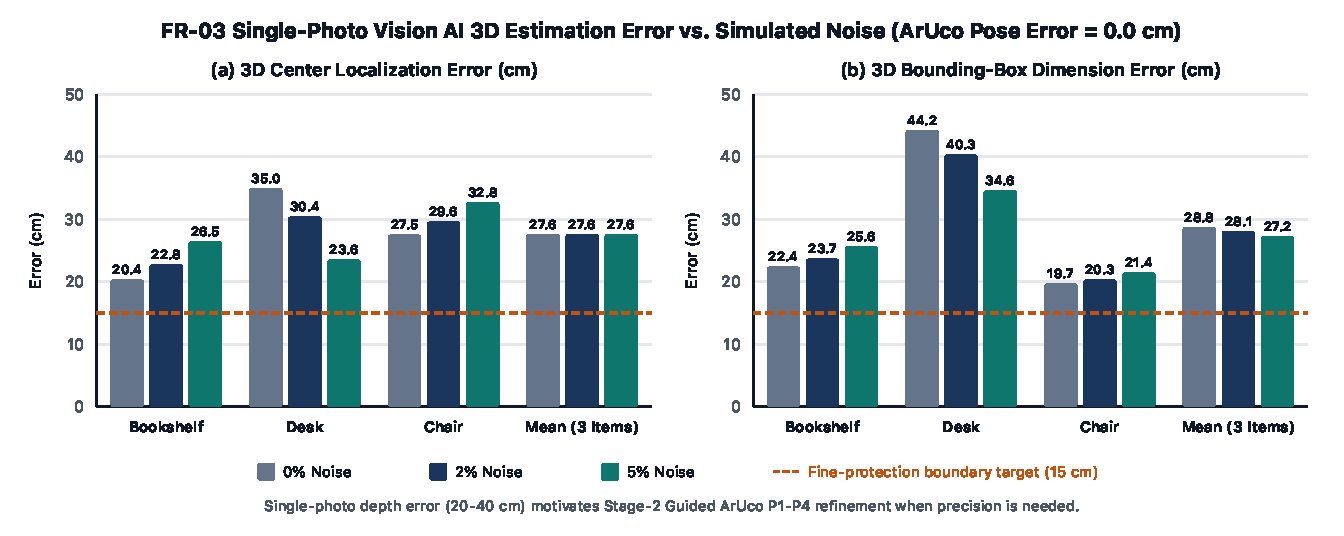
\includegraphics[width=0.80\textwidth]{figures/fig3_fr03_vision_3d_error.pdf}
\caption{Single-photo Vision AI 3D center localization error (a) and bounding-box dimension error (b) across 0\%, 2\%, and 5\% simulated noise (\texttt{run\_fr03\_vision\_3d\_experiment.py}; ArUco camera pose recovery error $= 0.0\text{ cm}$).}
\label{fig:fr03_err}
\end{figure*}

\section{Evaluation and Analysis}

\subsection{FR-01 Solar Nowcasting Evaluation}
Fig.~\ref{fig:fr01_err} and Table~\ref{tab:fr01_eval} compare frozen V1 against archived Open-Meteo forecasts on identical valid timestamps across Validation (Oct.~29--30) and the one-time Frozen Final Test (Nov.~2--5).

\textbf{Horizon Crossover and Operational Policy.} On the untouched Final Test, KMA V1 reduces MAE by \textbf{56.2\%} at 10~minutes ($73.16$ vs.\ $167.19\text{ W/m}^2$; bias $-2.57$ vs.\ $-90.16\text{ W/m}^2$) and \textbf{26.8\%} at 30~minutes ($122.30$ vs.\ $167.16\text{ W/m}^2$), with 10-minute PICP hitting 81.1\% against the 80\% nominal target. By 60~minutes, point persistence decays without spatial cloud-motion vectors and Open-Meteo catches up ($173.25$ vs.\ $177.54\text{ W/m}^2$), directly motivating our operational serving policy (V1 at 10 and 30~minutes, Open-Meteo at 60~minutes).

\textbf{Training Volume and Regime Breakdown.} Expanding training history from 10~days (503 rows) to 24~days (1,266 rows) kept 10-minute validation PICP at 82.5\% while narrowing mean interval width by \textbf{13.5\%} ($315.23$ to $272.72\text{ W/m}^2$) and cutting $P_{10}$ pinball loss by \textbf{15.4\%}. Stratified validation analysis shows 10-minute MAE of $20.37\text{ W/m}^2$ under clear skies (0--20\% cloud, $n=37$, vs.\ Open-Meteo $186.06\text{ W/m}^2$) and $80.68\text{ W/m}^2$ under overcast skies (70--100\%, $n=53$, 90.6\% PICP), while error concentrates in broken partly cloudy transitions (20--70\%, $n=7$: MAE $144.58\text{ W/m}^2$, PICP 57.1\%) and low solar elevation (5--20$^\circ$, $n=21$: PICP 52.4\%). Fig.~\ref{fig:fr01_ts} illustrates how 10-minute V1 tracks an abrupt afternoon cloud drop on holdout day \texttt{2026-11-03} that hourly NWP misses.

\subsection{FR-03 Vision AI 3D Estimation Analysis}
\label{sec:fr03_eval}
Fig.~\ref{fig:fr03_err} and Table~\ref{tab:fr03_eval} report 3D localization and dimension accuracy across 0\%, 2\%, and 5\% simulated detection and depth noise in the synthetic reading room.

\begin{table}[t]
\caption{FR-03 Synthetic 3D Center / Dimension Error (cm; Yaw Error $= 0.0^\circ$)}
\label{tab:fr03_eval}
\centering
\renewcommand{\arraystretch}{1.08}
\begin{tabular}{@{}crrrrr@{}}
\toprule
\textbf{Noise} & \textbf{Pose} & \textbf{Bookshelf} & \textbf{Desk} & \textbf{Chair} & \textbf{Mean C / D} \\
\midrule
0.0\% & 0.0 & 20.4 / 22.4 & 35.0 / 44.2 & 27.5 / 19.7 & \textbf{27.6 / 28.8} \\
2.0\% & 0.0 & 22.8 / 23.7 & 30.4 / 40.3 & 29.6 / 20.3 & \textbf{27.6 / 28.1} \\
5.0\% & 0.0 & 26.5 / 25.6 & 23.6 / 34.6 & 32.8 / 21.4 & \textbf{27.6 / 27.2} \\
\bottomrule
\end{tabular}
\end{table}

\begin{figure*}[t]
\centering
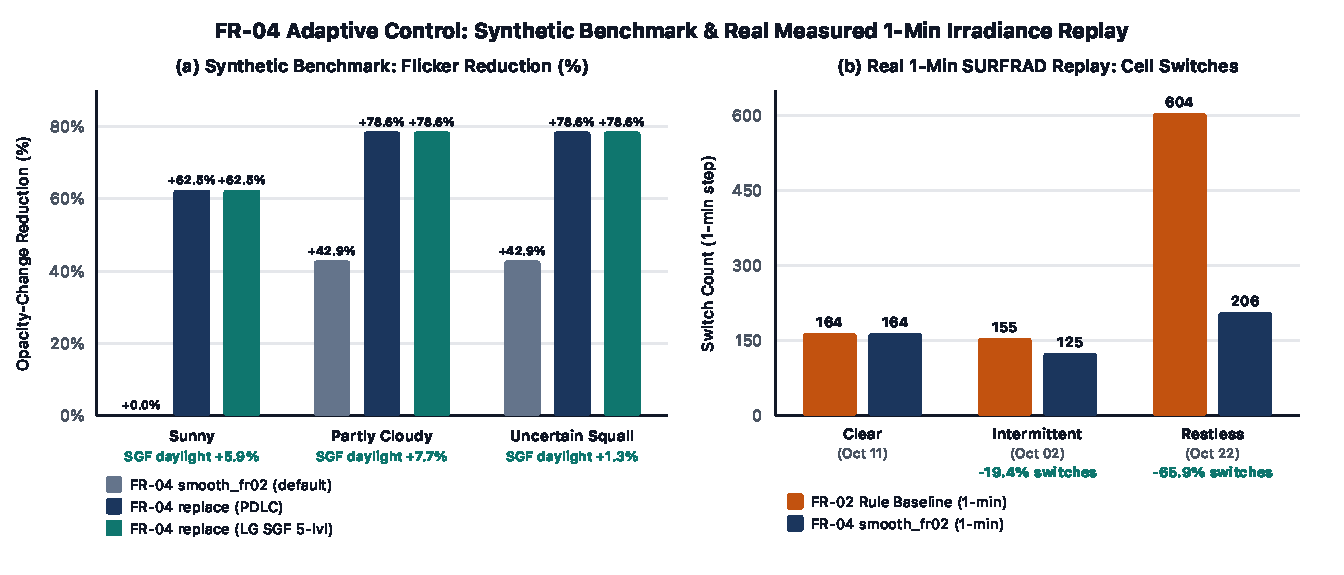
\includegraphics[width=0.80\textwidth]{figures/fig4_fr04_control_tradeoff.pdf}
\caption{(a) Total opacity-change (flicker) reduction and LG SGF sun-weighted Grade B daylight gain on synthetic stress scenarios; (b) Live API cell switch counts on real measured 1-minute NOAA SURFRAD irradiance days (\texttt{FR-02} versus default \texttt{FR-04 smooth\_fr02}).}
\label{fig:fr04_ctrl}
\end{figure*}

\begin{table*}[t]
\caption{FR-04 Synthetic Benchmark and Real-Weather API Replay Summary (Positive = Improvement Over FR-02)}
\label{tab:fr04_eval}
\centering
\footnotesize
\setlength{\tabcolsep}{4.5pt}
\renewcommand{\arraystretch}{1.10}
\begin{tabular}{@{}lcrrrr@{}}
\toprule
\textbf{Experiment and Mode / Day} & \textbf{Step} & \textbf{Flicker / Switch $\Delta$} & \textbf{Grade B / Same-Step} & \textbf{Sun-Wtd / vs.\ 30m} & \textbf{Cap $> q_{90}$} \\
\midrule
Synthetic: \texttt{smooth\_fr02} (default) & 5~min & $+0.0\%$ to $\mathbf{+42.9\%}$ & $-2.7\%$ to $+0.0\%$ & $-3.9\%$ to $+0.0\%$ & 9 / \textbf{0} \\
Synthetic: \texttt{replace} PDLC (binary) & 5~min & $+62.5\%$ to $\mathbf{+78.6\%}$ & $-3.5\%$ to $+0.0\%$ & $-3.9\%$ to $+0.8\%$ & 9 / \textbf{0} \\
Synthetic: \texttt{replace} LG SGF (5-lvl) & 5~min & $+62.5\%$ to $\mathbf{+78.6\%}$ & $-2.0\%$ to $+2.1\%$ & $\mathbf{+1.3\%}$ to $\mathbf{+20.6\%}$ & 9 / \textbf{0} \\
\midrule
Real KMA \texttt{2026-10-05} (restless) & 5~min & $\mathbf{+27.7\%}$ (159 $\to$ 115) & $-7.2\%$ & n/a & 0 / 0 \\
Real SURFRAD \texttt{2023-10-02} (interm.) & 1~min & $\mathbf{+19.4\%}$ (155 $\to$ 125) & $-0.7\%$ & $\mathbf{+31.5\%}$ vs.\ 30m & 0 / 0 \\
Real SURFRAD \texttt{2023-10-22} (restless) & 1~min & $\mathbf{+65.9\%}$ (604 $\to$ 206) & $-15.3\%$ & $\mathbf{+33.9\%}$ vs.\ 30m & 0 / 0 \\
\bottomrule
\end{tabular}
\end{table*}

Even at 0\% pixel noise, single-view 2D box unprojection retains a \textbf{27.6~cm} center and \textbf{28.8~cm} dimension floor (44.2~cm on the desk) due to class thickness priors ($0.40$--$0.70\text{ m}$). Initial real-photo diagnostics (\texttt{visualize\_fr03\_pipeline.py}) on rear/front chair photos ($s=0.13\text{ m}$) further exposed affine-shift compression in relative \texttt{Small-hf} ($Z=0.37$--$0.43\text{ m}$, width $0.20$--$0.22\text{ m}$), duplicate \texttt{tv}/\texttt{chair} boxes, and marker-corner false drops; switching to \texttt{Metric-Indoor-Small-hf} (99.2~MB) cut calibration RMSE 72--76\% ($3.90\to 0.92\text{ cm}$, $12.96\to 3.61\text{ cm}$) and sped CPU depth 4--8$\times$ ($275$--$541\text{ ms}$).

\textbf{Real-Room Cross-Family Depth Benchmark (\texttt{depthtest}).} To evaluate generalization against tape-measured room geometry, we benchmarked six Depth Anything V2 variants and five non-DA depth families (Apple Depth Pro \cite{b11}, DPT-Hybrid-MiDaS \cite{b12}, DPT-SwinV2-Tiny \cite{b12}, ZoeDepth-NYU \cite{b13}, and GLPN-NYU \cite{b14}) across all five \texttt{depthtest} images (Fig.~\ref{fig:fr03_bench}, Table~\ref{tab:depthtest_models}). Under EXIF $f_x$ and Oracle 2D boxes ($N=6$ primary targets), calibration design outweighed backbone size: switching \texttt{DA-V2 Metric-Small} from 4-corner affine ($0.562\text{ m}$) to proportional scaling ($\beta=0$) reduced front MAE by \textbf{56.6\%} to $0.244\text{ m}$ ($0.253\text{ m}$ with inner-60\% marker median), whereas upgrading to \texttt{Metric-Large} under affine ($0.469\text{ m}$, $10.8\times$ slower, $5{,}542\text{ MB}$ RSS) saved only $0.093\text{ m}$. No lightweight non-DA model outperformed \texttt{DA-V2 Metric-Small} within our 1.9~GB CPU budget: \texttt{DPT-SwinV2-Tiny} ($167\text{ ms}$, $1{,}336\text{ MB}$) scored $0.450\text{ m}$, and \texttt{GLPN-NYU} ($2{,}271\text{ ms}$, $1{,}851\text{ MB}$) scored $0.416\text{ m}$ raw ($0.545\text{ m}$ affine). \texttt{Apple Depth Pro} achieved the strongest non-DA center accuracy ($0.185\text{ m}$, $1.57\text{ cm}$ marker residual) and recovered focal length without EXIF at \textbf{6.13\%} mean absolute error (vs.\ 72.67\% hardcoded), confirming the value of FOV-aware metric depth, though its $5{,}887\text{ MB}$ RSS and $>195\text{ s}$ CPU time require GPU hosting.

\textbf{Condition Ablation and Live Post-Fix Production Verification.} Condition-wise ablation exposed four root causes: (1) hardcoded $f_x = 0.9\max(w, h)$ pushed 4/5 cameras outside the room ($3.509\text{ m}$ 3D drift on 0.5$\times$ ultrawide), while a radial sweep ($k_1 \in [-0.20, +0.10]$) proved $k_1=0.0$ is optimal ($0.31$ and $0.19\text{ px}$ reprojection), confirming smartphone ISPs already rectify barrel distortion; once EXIF $f_x$ and proportional calibration were applied, 0.5$\times$ beat 1$\times$ ($0.088\text{ m}$ vs.\ $0.350\text{ m}$ front MAE under $S_3$) because all four desk corners remained visible; (2) \texttt{otherside} photos produced four glass-wall hallway chair FPs ($x=3.63$--$8.10\text{ m}$) dragged $1.02$--$5.26\text{ m}$ inward by clamping, and occluded chair backrests gave $0.421\text{ m}$ height MAE under $p_{\mathrm{top}}-p_{\mathrm{bot}}$ vs.\ $0.033\text{ m}$ under floor-referenced $p_{\mathrm{top,ENU},z}$; (3) raising YOLO \texttt{conf\_thresh} from $0.25$ to $0.35$ halved desk recall ($4/4 \to 2/4$) without removing TV/hallway FPs, justifying deterministic geometric filters; and (4) single-$Z$ back-projection locked cuboid yaw to camera $+X$ ($34.2^\circ$ mean error) and fixed desk depth to $0.70\text{ m}$ ($1.08\text{ m}$ error).

Table~\ref{tab:depthtest_postfix} and Figs.~\ref{fig:fr03_desk}--\ref{fig:fr03_twochair} verify the actual modified \texttt{VisionRegistrationPipeline} live on all five \texttt{depthtest} photos (\texttt{post\_fix\_eval.json}, 0~MB extra neural weight): live E2E wall-normal front MAE drops \textbf{65.3\%} ($0.557 \to 0.193\text{ m}$), center MAE drops \textbf{69.4\%} ($0.490 \to 0.150\text{ m}$), desk depth MAE drops \textbf{62.6\%} ($1.105 \to 0.413\text{ m}$), desk 2D footprint IoU rises \textbf{69.0\%} ($0.289 \to 0.489$; $0.511$ with Oracle 2D), \texttt{twochair} front MAE drops \textbf{90.1\%} ($1.216 \to 0.121\text{ m}$), 5/5 cameras resolve inside the room (EXIF-stripped 0.5$\times$ \texttt{distortion\_otherside} auto-recovers $f_x = 1584.6\text{ px}$ within 1.06\% of true $1568.0\text{ px}$ at $0.05\text{ px}$ reprojection), primary clamping drops to 0, and 10/11 (90.9\%) confirmed FPs are eliminated (0 TV, 0 laptop-as-bookshelf, 1 hallway chair within the 25~cm glass-wall margin).

\begin{table}[!tb]
\caption{Live Post-Fix Production Verification on \texttt{depthtest} (\texttt{post\_fix\_eval.json})}
\label{tab:depthtest_postfix}
\centering
\scriptsize
\setlength{\tabcolsep}{3.0pt}
\renewcommand{\arraystretch}{1.08}
\begin{tabular}{@{}lrrr@{}}
\toprule
\textbf{Metric (DA-V2-M-Small + YOLO)} & \textbf{Pre-Fix} & \textbf{Post-Fix} & \textbf{Delta} \\
\midrule
Cameras inside room & 1 / 5 & \textbf{5 / 5} & $+80\%$p \\
Mean IPPE reproj.\ error & 5.75~px & \textbf{1.04~px} & $-81.9\%$ \\
Primary Front MAE & 0.557~m & \textbf{0.193~m} & $\mathbf{-65.3\%}$ \\
Primary Center MAE & 0.490~m & \textbf{0.150~m} & $\mathbf{-69.4\%}$ \\
Desk-4 Depth MAE & 1.105~m & \textbf{0.413~m} & $\mathbf{-62.6\%}$ \\
Desk-4 2D Footprint IoU & 0.289 & \textbf{0.489} & $\mathbf{+69.0\%}$ \\
\texttt{twochair} Front MAE & 1.216~m & \textbf{0.121~m} & $\mathbf{-90.1\%}$ \\
Confirmed FPs (TV/book/hall) & 11 & \textbf{1} & $\mathbf{-90.9\%}$ \\
Oracle 2D Front / IoU ($N=6$) & 0.562 / 0.285 & \textbf{0.216 / 0.511} & $-61.6\%$ \\
\bottomrule
\end{tabular}
\end{table}

\textbf{Unconstrained Colab GPU Optimal Upper Bound (Tesla T4).} To measure the accuracy ceiling of our architecture without the 1.9~GB CPU RAM limit, we ran a 91-combination benchmark on a Google Colab NVIDIA Tesla T4 GPU ($14{,}912.7\text{ MB}$ VRAM, CUDA 13.0, PyTorch 2.14.1). Running the fixed CPU production stack on T4 matched CPU metrics within 0.1--0.2~mm ($0.1933\text{ m}$ front, $0.1501\text{ m}$ center, $0.4892$ IoU) at $371.0\text{ ms}$ ($3.2\times$ faster). Larger YOLO variants (\texttt{YOLO11x}, \texttt{YOLO11x-seg}, \texttt{YOLOv8x-seg}) separated \texttt{twochair} (2/2) but collapsed conference-desk recall ($1/4$ and $0/4$ desks), whereas global-attention \texttt{RT-DETR-x} \cite{b15} ($109.8\text{ ms}$, $625.8\text{ MB}$) achieved \textbf{6/6 primary and 15/15 all-visible recall}. Prompting \texttt{SAM 2.1 Base} \cite{b16} ($690.8\text{ MB}$) with \texttt{RT-DETR-x} boxes feeds pixel-exact masks into our 3D ENU point-cloud fitter (Fig.~\ref{fig:fr03_gpu_opt}, Fig.~\ref{fig:fr03_gpu_twochair}, Table~\ref{tab:depthtest_gpu}): paired with \texttt{DA-V2 Metric-Small} (\texttt{Zero-FP Mask GPU}), confirmed FPs drop to \textbf{0} ($0.1586\text{ m}$ front, $0.0978\text{ m}$ center, $0.5967$ IoU, $\approx 1.5\text{ GB}$ VRAM); paired with \texttt{Apple Depth Pro} (\texttt{fp16}, $4{,}773.7\text{ MB}$ simultaneous VRAM), the winning GPU stack reaches \textbf{6/6 recall, $0.1032\text{ m}$ front MAE, $0.0728\text{ m}$ center MAE, $0.6763$ desk IoU, $1.8\text{ cm}$ desk height MAE, and $3.7\text{ cm}$ \texttt{twochair} front MAE} ($0.0945\text{ m}$ front and $0.0323\text{ m}$ \texttt{twochair} even in pure EXIF-free \texttt{depthpro\_pred\_fx} mode with 5/5 cameras inside the room).

\begin{figure*}[!tbp]
\centering
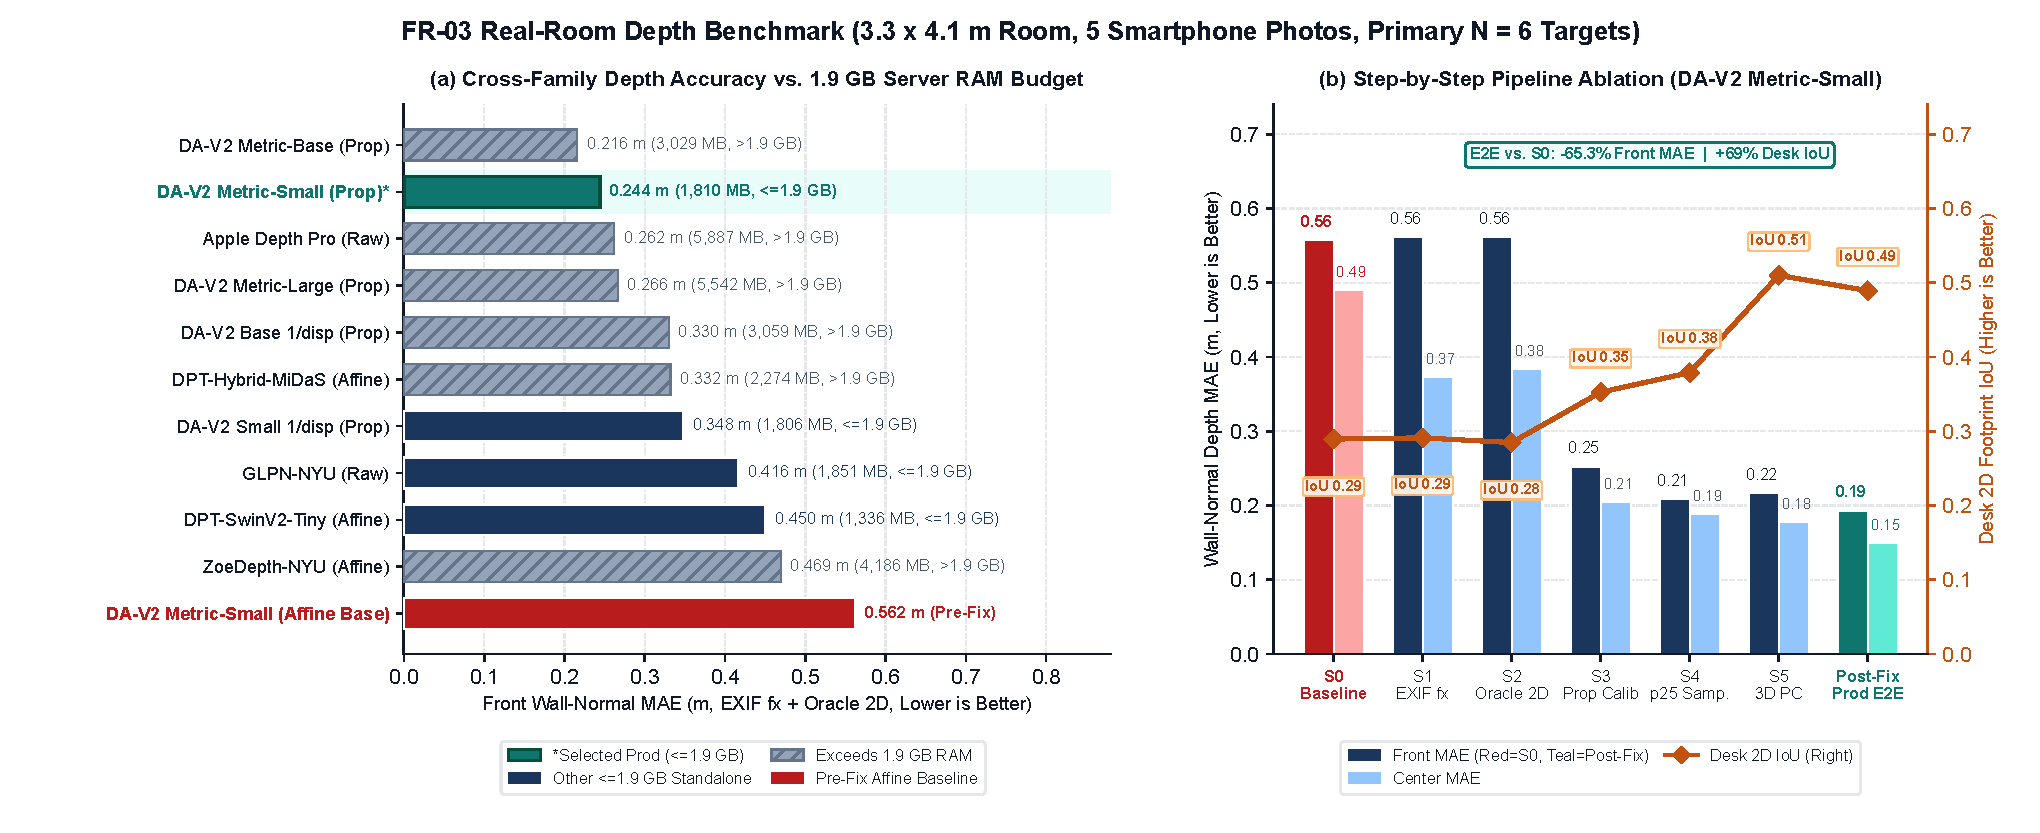
\includegraphics[width=0.86\textwidth]{figures/fig5_fr03_depthtest_benchmark.pdf}
\caption{Real-room \texttt{depthtest} benchmark ($3.30 \times 4.10 \times 2.50\text{ m}$, $N=6$ primary targets): (a) cross-family monocular depth accuracy (EXIF $f_x$ + Oracle 2D) versus isolated peak RSS against the 1.9~GB AWS CPU budget; (b) step-by-step ablation waterfall from pre-fix baseline ($S_0$) to the live verified post-fix production pipeline (\texttt{post\_fix\_eval.json}: $-65.3\%$ front MAE, $+69.0\%$ desk 2D footprint IoU).}
\label{fig:fr03_bench}
\end{figure*}

\begin{figure*}[!tbp]
\centering
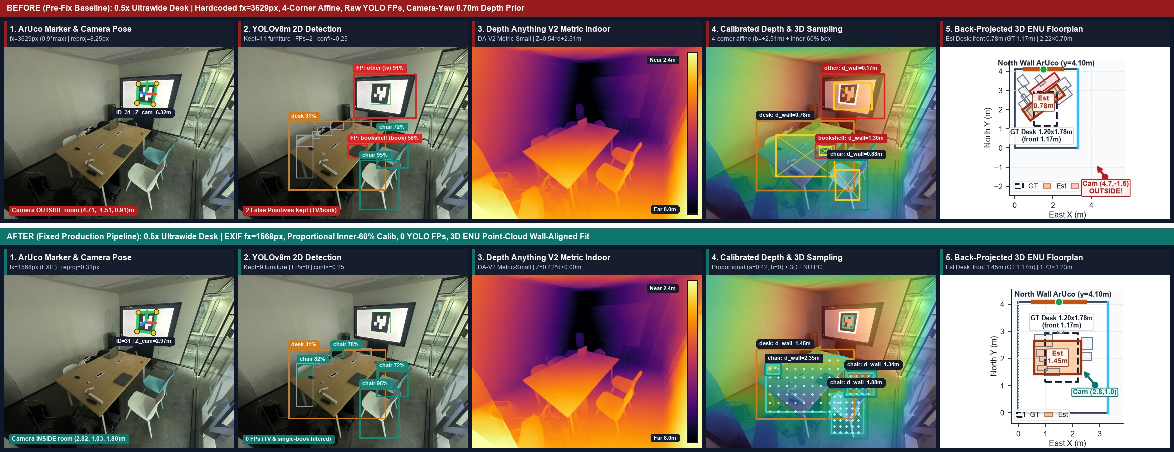
\includegraphics[width=0.88\textwidth]{figures/fig6_fr03_5stage_comparison_desk.pdf}
\caption{Live 5-stage Before (top) versus After (bottom) comparison on \texttt{depthtest\_distortion.jpeg} (0.5$\times$ ultrawide desk, \texttt{ID=31}, $s=0.60\text{ m}$). Post-fix production code recovers EXIF $f_x = 1568\text{ px}$ ($0.31\text{ px}$ reprojection, camera inside room), removes TV and laptop-as-book false positives, applies proportional ArUco calibration ($\alpha=0.42, \beta=0$), and fits a wall-aligned 3D ENU point-cloud desk (center $2.07\text{ m}$ vs.\ GT $2.06\text{ m}$, IoU $0.53$).}
\label{fig:fr03_desk}
\end{figure*}

\begin{figure*}[!tbp]
\centering
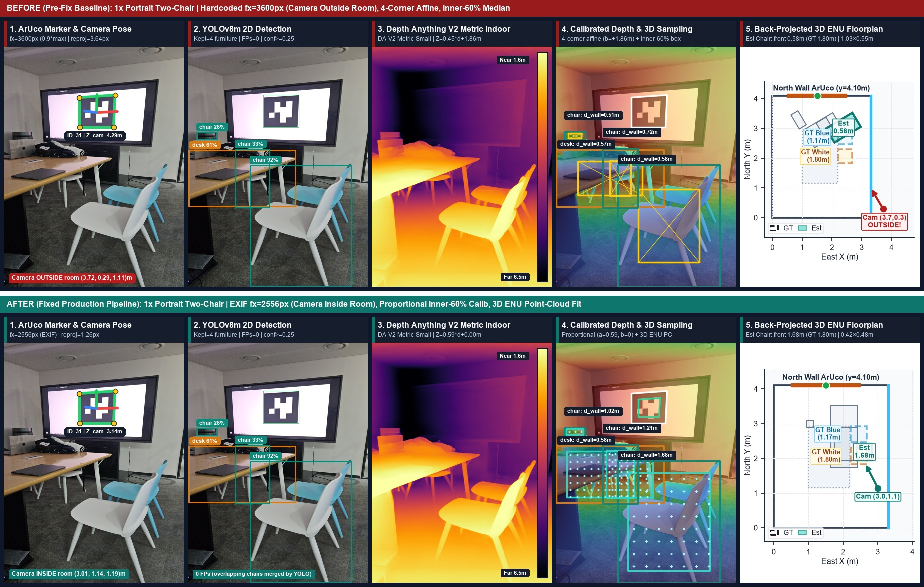
\includegraphics[width=0.78\textwidth]{figures/fig7_fr03_5stage_comparison_twochair.pdf}
\caption{Live 5-stage Before (top) versus After (bottom) comparison on \texttt{depthtest\_twochair.jpeg} ($2252 \times 4000$, \texttt{ID=31}, $s=0.60\text{ m}$). Replacing hardcoded $f_x=3600\text{ px}$ and 4-corner affine extrapolation ($\beta=+1.86\text{ m}$) with EXIF $f_x=2556\text{ px}$, proportional calibration, and 3D ENU point-cloud filtering reduces chair front error by 90.1\% ($0.58 \to 1.68\text{ m}$ vs.\ GT $1.80\text{ m}$) and restores footprint dimensions ($0.42 \times 0.48\text{ m}$ vs.\ GT $0.47 \times 0.46\text{ m}$).}
\label{fig:fr03_twochair}
\end{figure*}

\begin{table*}[!tbp]
\caption{Real-Room \texttt{depthtest} Cross-Family Monocular Depth Benchmark (EXIF $f_x$ + Oracle 2D, Primary $N=6$)}
\label{tab:depthtest_models}
\centering
\scriptsize
\setlength{\tabcolsep}{3.6pt}
\renewcommand{\arraystretch}{1.08}
\begin{tabular}{@{}llrrrrrl@{}}
\toprule
\textbf{Model (Type)} & \textbf{Calib.} & \textbf{Front MAE} & \textbf{Center MAE} & \textbf{Mkr RMSE} & \textbf{Latency} & \textbf{Peak RSS} & \textbf{1.9~GB CPU Server} \\
\midrule
DA-V2 Metric-Base (Metric) & Prop ($\beta=0$) & \textbf{0.216~m} & 0.203~m & 0.091~m & 754~ms & 3,029~MB & Infeasible (OOM) \\
\textbf{DA-V2 Metric-Small (Selected)} & \textbf{Prop ($\beta=0$)} & \textbf{0.244~m} & 0.205~m & 0.075~m & \textbf{321~ms} & \textbf{1,810~MB} & \textbf{Standalone Feasible} \\
Apple Depth Pro (Metric+FOV) & Raw / Calib & 0.262 / 0.268~m & \textbf{0.195 / 0.185~m} & \textbf{0.016~m} & 2,568~ms (MPS) & 5,887~MB & Infeasible (GPU req.) \\
DA-V2 Metric-Large (Metric) & Prop ($\beta=0$) & 0.266~m & 0.230~m & 0.071~m & 3,481~ms & 5,542~MB & Infeasible (OOM) \\
DA-V2 Base 1/disp (Relative) & Prop ($\beta=0$) & 0.330~m & 0.247~m & 0.139~m & 771~ms & 3,059~MB & Infeasible (OOM) \\
DPT-Hybrid-MiDaS (Relative) & Affine & 0.332~m & 0.290~m & 0.101~m & 509~ms & 2,274~MB & Infeasible (OOM risk) \\
DA-V2 Small 1/disp (Relative) & Prop ($\beta=0$) & 0.348~m & 0.253~m & 0.156~m & 324~ms & 1,806~MB & Standalone Feasible \\
GLPN-NYU (Metric NYU) & Raw / Affine & 0.416 / 0.545~m & 0.287 / 0.459~m & 0.132~m & 2,271~ms & 1,851~MB & Marginal / Slow \\
DPT-SwinV2-Tiny (Relative) & Affine & 0.450~m & 0.341~m & 0.032~m & \textbf{167~ms} & \textbf{1,336~MB} & Feasible (Low acc.) \\
ZoeDepth-NYU (Metric NYU) & Affine & 0.469~m & 0.325~m & 0.046~m & 1,173~ms & 4,186~MB & Infeasible (OOM) \\
DA-V2 Metric-Small (Pre-Fix) & Affine & 0.562~m & 0.384~m & 0.039~m & 321~ms & 1,810~MB & Baseline (Buggy fit) \\
\bottomrule
\end{tabular}
\end{table*}

\begin{figure*}[!tbp]
\centering
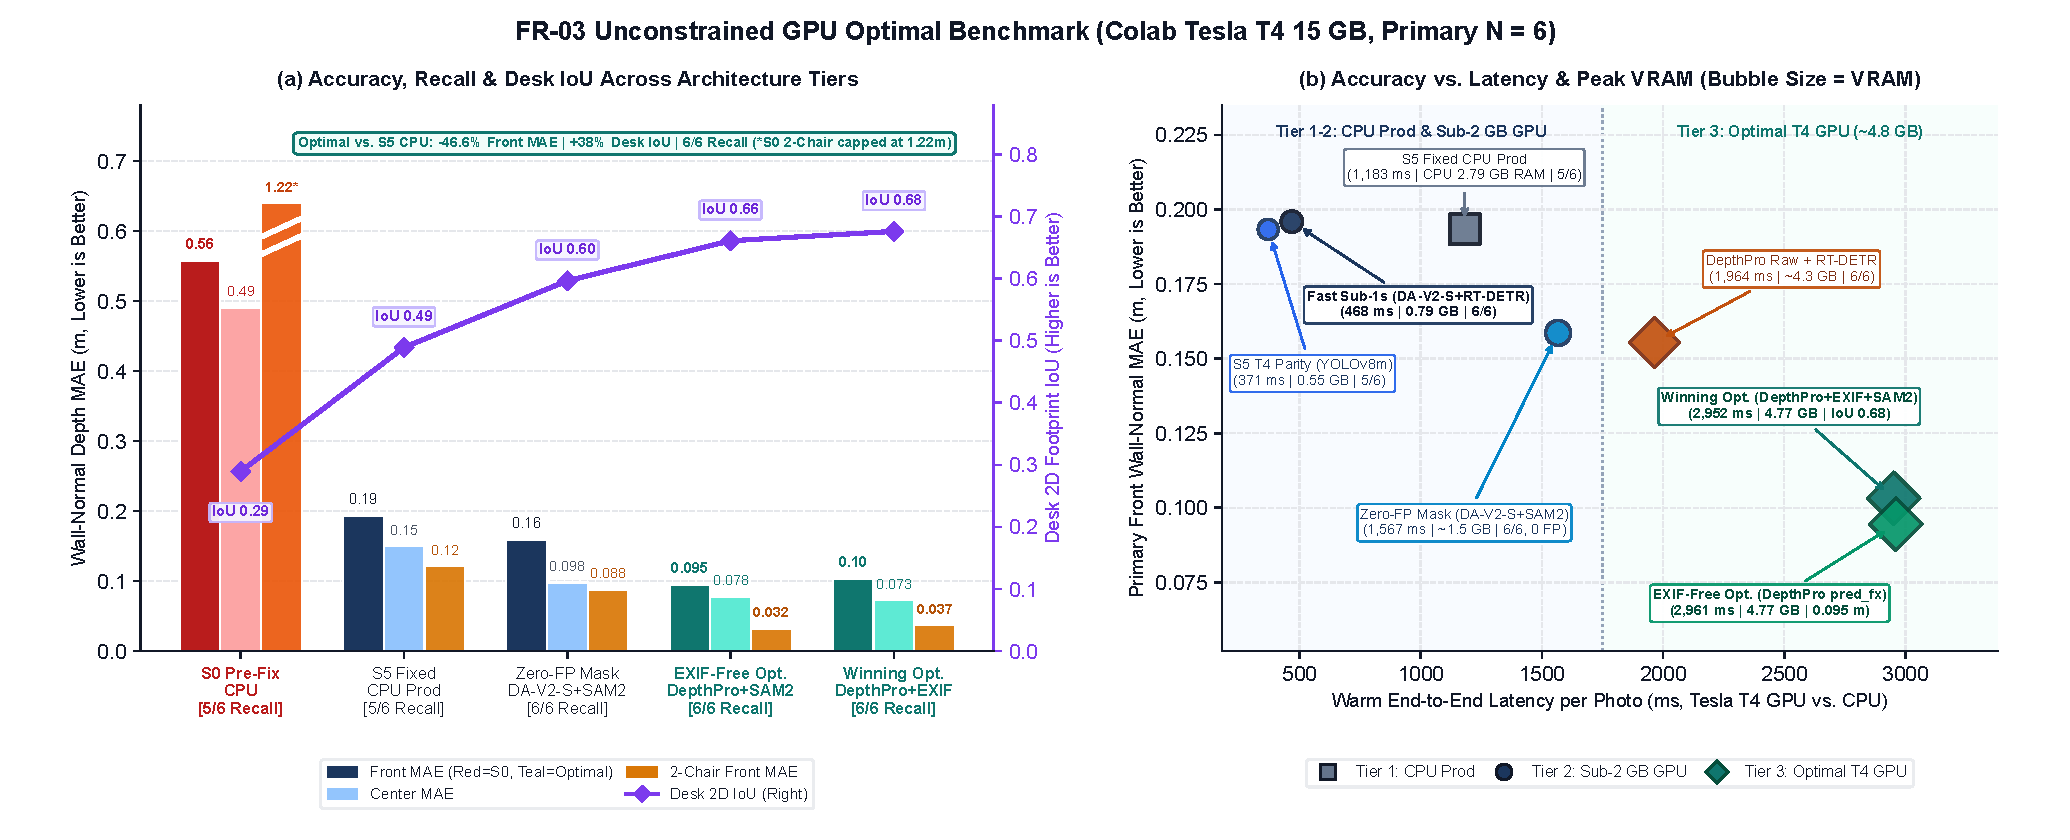
\includegraphics[width=0.86\textwidth]{figures/fig8_fr03_colab_gpu_optimal.pdf}
\caption{Colab Tesla T4 unconstrained GPU optimal benchmark ($N=6$ primary targets, \texttt{colab\_optimal\_summary.json}): (a) accuracy and desk 2D IoU progression from pre-fix CPU ($S_0$) through fixed CPU production ($S_5$) to T4 GPU optimal stacks (6/6 recall, $0.095$--$0.103\text{ m}$ front MAE, $0.676$ desk IoU); (b) accuracy versus warm E2E latency and allocated VRAM across three deployment tiers (CPU Prod, Sub-2~GB GPU, Optimal T4 GPU).}
\label{fig:fr03_gpu_opt}
\end{figure*}

\begin{figure*}[!tbp]
\centering
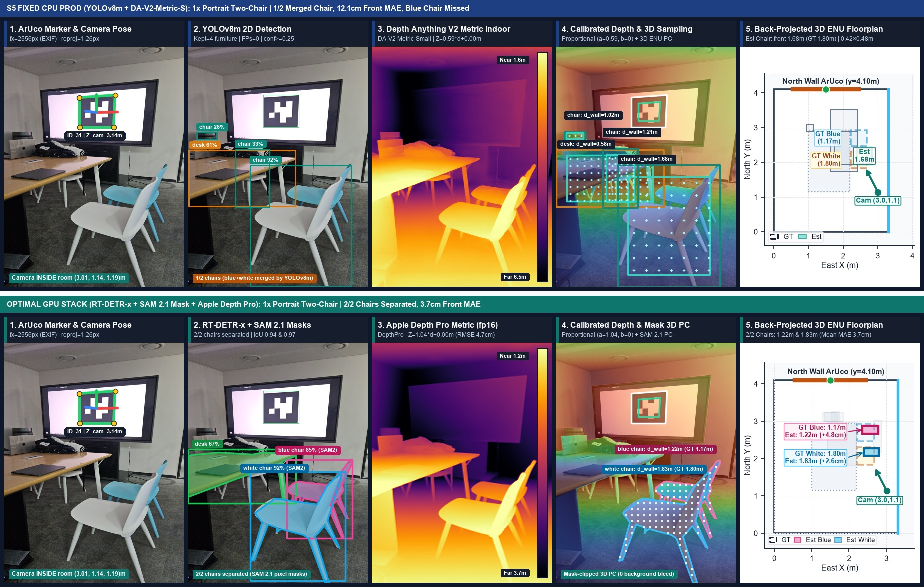
\includegraphics[width=0.76\textwidth]{figures/fig9_fr03_5stage_gpu_optimal_twochair.pdf}
\caption{Live 5-stage visual comparison on \texttt{depthtest\_twochair.jpeg}: Tier-1 Fixed CPU Production (\texttt{YOLOv8m + DA-V2-Metric-S}, top: 1/2 merged chair, $12.1\text{ cm}$ front MAE) versus Tier-3 Optimal GPU Stack (\texttt{RT-DETR-x + SAM 2.1 Base + Apple Depth Pro}, bottom: 2/2 chairs separated via pixel-exact SAM 2.1 masks, IoU $0.94/0.97$, blue $1.22\text{ m}$ vs.\ GT $1.17\text{ m}$ and white $1.83\text{ m}$ vs.\ GT $1.80\text{ m}$, $3.7\text{ cm}$ mean front MAE).}
\label{fig:fr03_gpu_twochair}
\end{figure*}

\begin{table*}[!tbp]
\caption{End-to-End CPU vs.\ Colab Tesla T4 GPU Optimal Stack Comparison and 3-Tier Deployment Summary (\texttt{depthtest})}
\label{tab:depthtest_gpu}
\centering
\scriptsize
\setlength{\tabcolsep}{3.4pt}
\renewcommand{\arraystretch}{1.08}
\begin{tabular}{@{}lcrrrrrrl@{}}
\toprule
\textbf{Pipeline Stack} & \textbf{Recall} & \textbf{Front MAE} & \textbf{Center MAE} & \textbf{Desk IoU} & \textbf{2-Chair F.} & \textbf{FP} & \textbf{Warm Lat.} & \textbf{Peak Mem. / Tier} \\
\midrule
$S_0$ Pre-Fix CPU Baseline & 5/6 & 0.5572~m & 0.4902~m & 0.2895 & 1.2162~m & 11 & $\sim$1,180~ms & CPU / Baseline \\
$S_5$ Fixed CPU Prod (\texttt{DA-V2-S+YOLOv8m}) & 5/6 & 0.1934~m & 0.1499~m & 0.4893 & 0.1209~m & 1 & 1,182.5~ms & 2,794~MB RAM (Tier 1) \\
$S_5$ T4 GPU Parity (\texttt{DA-V2-S+YOLOv8m}) & 5/6 & 0.1933~m & 0.1501~m & 0.4892 & 0.1208~m & 1 & \textbf{371.0~ms} & 549~MB VRAM (Parity) \\
Fast Sub-1s GPU (\texttt{DA-V2-S+RT-DETR-x}) & \textbf{6/6} & 0.1959~m & 0.1748~m & 0.4998 & 0.1211~m & 1 & \textbf{468.0~ms} & \textbf{789~MB} (Tier 2 GPU) \\
Zero-FP Mask GPU (\texttt{DA-V2-S+RT-DETR+SAM2}) & \textbf{6/6} & 0.1586~m & 0.0978~m & 0.5967 & 0.0880~m & \textbf{0} & 1,566.8~ms & $\sim$1.5~GB (Tier 2 GPU) \\
DepthPro Raw + \texttt{RT-DETR-x} ($\alpha=1.0$) & \textbf{6/6} & 0.1554~m & 0.1491~m & 0.5159 & 0.0895~m & 2 & 1,964.2~ms & 4,388~MB (Ablation) \\
EXIF-Free Opt.\ (\texttt{DepthPro pred\_fx+SAM2}) & \textbf{6/6} & \textbf{0.0945~m} & 0.0777~m & 0.6612 & \textbf{0.0323~m} & 2 & 2,960.8~ms & 4,774~MB (Tier 3 GPU) \\
\textbf{Winning Opt.\ GPU (\texttt{DepthPro+EXIF+SAM2})} & \textbf{6/6} & \textbf{0.1032~m} & \textbf{0.0728~m} & \textbf{0.6763} & \textbf{0.0370~m} & 2 & 2,951.6~ms & 4,774~MB (Tier 3 GPU) \\
\bottomrule
\end{tabular}
\end{table*}

\subsection{FR-04 Adaptive Control and Real-Weather Replay}
Fig.~\ref{fig:fr04_ctrl} and Table~\ref{tab:fr04_eval} summarize both the 4-scenario synthetic stress benchmark and live-API real-weather replays on KMA GK2A and 1-minute NOAA SURFRAD streams.

In the synthetic suite, all three FR-04 modes eliminated all 9 baseline $q_{90}$ cap exceedances, while 5-level LG SGF dimming matched PDLC's $+78.6\%$ flicker reduction and gained $+1.3\%$ to $+20.6\%$ more sun-weighted Grade B daylight. On real measured 1-minute SURFRAD data, default \texttt{smooth\_fr02} cut restless-day switches by \textbf{65.9\%} (604 down to 206) while admitting \textbf{+31.5\% to +33.9\% more daylight} than coarse 30-minute FR-02 schedules (mean opacity $0.0805$ vs.\ $0.1217$ on Oct.~22). At 10-minute or 30-minute steps, single intervals already meet or exceed the $600\text{ s}$ gap-fill and holding limits, leaving no sub-step flicker for \texttt{smooth\_fr02} to suppress.

\subsection{Automated Verification}
The automated regression suite passes \textbf{856 / 856} baseline backend/engine \texttt{pytest} tests plus \textbf{8 new Vision AI P0/P1 regression tests} (\textbf{102 / 102} passed across Vision AI, window-marker, and film-clamping suites; \texttt{ruff check}, \texttt{ruff format --check}, \texttt{mypy} on 78 files, and \texttt{app.scene\_cli schema --check} all pass with 0 errors) and \textbf{207 / 207} frontend unit tests (\texttt{node --test}), verifying anti-leakage splits, frozen artifact fidelity, EXIF/1D-focal recovery, proportional single-marker calibration, 3D ENU point-cloud fitting, non-destructive clamping, \texttt{mode=experiment} diagnostics, \texttt{VisionPreview} geometry, real-weather replays, and rolling scenario precomputation.

\section{Related Work and Tools}

Our solar prior uses the Erbs, Klein, and Duffie diffuse-fraction model \cite{b1} via \texttt{pvlib} \cite{b4}, and follows probabilistic solar forecasting practice using quantile pinball loss and PICP \cite{b2,b3}. Window-marker pose recovery applies Infinitesimal Plane-Based Pose Estimation for planar squares (\texttt{SOLVEPNP\_IPPE\_SQUARE}) \cite{b5}, combined with Depth Anything V2 \cite{b6} for indoor metric depth (benchmarked against Depth Pro \cite{b11}, DPT/MiDaS \cite{b12}, ZoeDepth \cite{b13}, and GLPN \cite{b14}) and Ultralytics YOLOv8 \cite{b7} on CPU (evaluated against RT-DETR \cite{b15} and SAM 2 \cite{b16} on GPU).

The production stack integrates \texttt{pvlib}, \texttt{NumPy}, \texttt{SciPy} (L-BFGS-B), \texttt{Shapely}, \texttt{OpenCV}, \texttt{Ultralytics}, \texttt{PyTorch}, \texttt{HuggingFace Transformers}, \texttt{FastAPI}, \texttt{Pydantic v2}, \texttt{SQLModel}, WAL-mode \texttt{SQLite}, \texttt{React}, \texttt{TypeScript}, \texttt{Vite}, and \texttt{Three.js}, consuming KMA GK2A \cite{b8}, Open-Meteo \cite{b9}, and NOAA SURFRAD \cite{b10} data while targeting LG Chem SGF and LG ThinQ ON smart-home integration.

\section{Conclusion and Discussion}

SunSync-AI demonstrates an end-to-end prototype unifying sub-hourly probabilistic solar nowcasting, marker-anchored hybrid Vision 3D sensing, and flicker-stabilized smart window control. Frozen linear quantile regression reduced 10-minute and 30-minute DNI MAE by 56.2\% and 26.8\% on a strict holdout test while deferring 60-minute horizons to Open-Meteo. Real-room \texttt{depthtest} evaluation across 11 monocular depth variants and four capture conditions guided production P0/P1 fixes (EXIF and 1D focal search, proportional single-marker scaling, deterministic FP gates, 3D ENU point-cloud wall-aligned cuboids, floor height, and non-destructive clamping) that cut live E2E wall-normal depth MAE by 65.3\% ($0.557\to 0.193\text{ m}$), lifted desk 2D IoU by 69.0\% ($0.289\to 0.489$), and removed 90.9\% of confirmed FPs at zero extra model weight, while an unconstrained Google Colab Tesla T4 GPU benchmark (\texttt{RT-DETR-x + SAM 2.1 Base + Apple Depth Pro}) established a 6/6 recall, $9.5$--$10.3\text{ cm}$ front MAE ($3.2$--$3.7\text{ cm}$ on \texttt{twochair}), and $0.676$ desk IoU accuracy ceiling across three deployment tiers, paired with Stage-2 guided \texttt{P1}--\texttt{P4} ArUco refinement. Adaptive FR-04 control cut cell switches by up to 65.9\% on restless measured 1-minute skies while admitting over 31\% more daylight than 30-minute rule schedules, supported by 10-minute rolling scenario precomputation.

\textbf{Limitations and Future Work.} Four constraints merit ongoing work: (1) FR-01 data covers one Seoul autumn month using Erbs \texttt{dsr\_proxy} rather than collocated pyrheliometer DNI; (2) \texttt{advection\_impact} remains $0.0$ in V1, contributing to lower PICP (57.1\%) during partly cloudy transitions until GK2A 2D cloud-motion patches are added; (3) in real-room Vision AI, overlapping line-of-sight objects (\texttt{twochair}) still merge into one YOLOv8m box, one hallway chair within 25~cm of the glass wall passed the room buffer, and co-loading YOLOv8m with DA-V2 Metric-Small reached 2,794~MB peak RSS on macOS, motivating instance segmentation (\texttt{yolov8-seg}) or interactive box splitting, ONNX INT8 quantization / sequential execution on 1.9~GB CPU servers, and multi-room field validation; and (4) 1-minute FR-04 replays borrow Pennsylvania SURFRAD skies with assumed LG SGF transmittance ($0.03$--$0.72$), while dashboard badges preview at 30-minute steps.

\begin{thebibliography}{00}
\bibitem{b1} D. G. Erbs, S. A. Klein, and J. A. Duffie, ``Estimation of the diffuse radiation fraction for hourly, daily and monthly-average global radiation,'' \textit{Solar Energy}, vol. 28, no. 4, pp. 293--302, 1982.
\bibitem{b2} D. W. van der Meer, J. Wid\'{e}n, and J. Munkhammar, ``Review on probabilistic forecasting of photovoltaic power production and electricity consumption,'' \textit{Renewable and Sustainable Energy Reviews}, vol. 81, pp. 1484--1512, 2018.
\bibitem{b3} P. Lauret, M. David, and H. T. C. Pedro, ``Probabilistic solar forecasting using quantile regression models,'' \textit{Energies}, vol. 10, no. 10, p. 1591, 2017.
\bibitem{b4} W. F. Holmgren, C. W. Hansen, and M. A. Mikofski, ``pvlib python: a python package for modeling solar energy systems,'' \textit{Journal of Open Source Software}, vol. 3, no. 29, p. 884, 2018.
\bibitem{b5} T. Collins and A. Bartoli, ``Infinitesimal plane-based pose estimation,'' \textit{International Journal of Computer Vision}, vol. 109, no. 3, pp. 252--286, 2014.
\bibitem{b6} L. Yang, B. Kang, Z. Huang, Z. Zhao, X. Xu, J. Feng, and H. Zhao, ``Depth Anything V2,'' \textit{Advances in Neural Information Processing Systems (NeurIPS)}, 2024.
\bibitem{b7} G. Jocher, A. Chaurasia, and J. Qiu, ``Ultralytics YOLOv8,'' 2023. [Online]. Available: \url{https://github.com/ultralytics/ultralytics}
\bibitem{b8} Korea Meteorological Administration (KMA), ``GK2A Satellite API Hub (DSR and Cloud Amount Products),'' 2026. [Online]. Available: \url{https://apihub.kma.go.kr}
\bibitem{b9} Open-Meteo, ``Historical Forecast API (ECMWF IFS 0.25-degree Single Runs),'' 2026. [Online]. Available: \url{https://open-meteo.com}
\bibitem{b10} NOAA Global Monitoring Laboratory, ``SURFRAD Surface Radiation Budget Network (Penn State, PA),'' 2023. [Online]. Available: \url{https://gml.noaa.gov/grad/surfrad/}
\bibitem{b11} A. Bochkovskii, A. Delaunoy, H. Germain, M. Santos, Y. Zhou, S. R. Richter, and V. Koltun, ``Depth Pro: Sharp monocular metric depth in less than a second,'' \textit{arXiv:2410.02073}, 2024.
\bibitem{b12} R. Ranftl, A. Bochkovskiy, and V. Koltun, ``Vision transformers for dense prediction,'' in \textit{Proc. IEEE/CVF Int. Conf. Computer Vision (ICCV)}, pp. 12179--12188, 2021.
\bibitem{b13} S. F. Bhat, R. Birkl, D. Wofk, P. Wonka, and M. M\"{u}ller, ``ZoeDepth: Zero-shot transfer by combining relative and metric depth,'' \textit{arXiv:2302.12288}, 2023.
\bibitem{b14} D. Kim, W. Ka, P. Ahn, D. Joo, S. Chun, and J. Kim, ``Global-local path networks for monocular depth estimation with vertical cutdepth,'' \textit{arXiv:2201.07436}, 2022.
\bibitem{b15} Y. Zhao, W. Lv, S. Xu, J. Wei, G. Wang, Q. Dang, Y. Liu, and J. Chen, ``DETRs beat YOLOs on real-time object detection,'' in \textit{Proc. IEEE/CVF Conf. Computer Vision and Pattern Recognition (CVPR)}, pp. 16965--16974, 2024.
\bibitem{b16} N. Ravi, V. Gabeur, Y.-T. Hu, R. Hu, C. Ryali, T. Ma, H. Khedr, R. R\"{a}dle, C. Rolland, L. Gustafson, E. Mintun, J. Pan, K. V. Alwala, N. Carion, C.-Y. Wu, R. Girshick, P. Doll\'{a}r, and C. Feichtenhofer, ``SAM 2: Segment anything in images and videos,'' \textit{arXiv:2408.00714}, 2024.
\end{thebibliography}

\end{document}
